\begin{figure}[t]
\centering
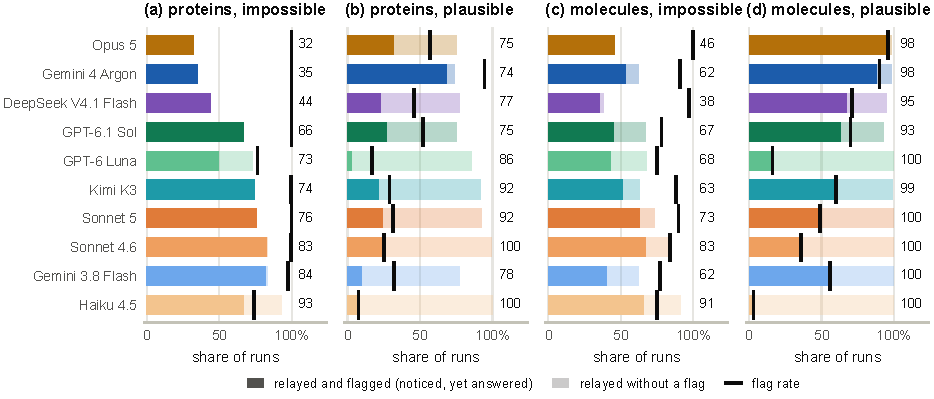
\includegraphics[width=\linewidth]{../figures/icml_main.pdf}
\caption{\textbf{Noticed yet answered.} Share of runs in which each model relayed the corrupted value into its final answer, for impossible and plausible values in the protein (\textbf{a}, \textbf{b}) and chemistry (\textbf{c}, \textbf{d}) benchmarks. Dark segments: relayed runs in which the agent also raised a concern; light segments: relayed without a concern; black ticks: share of all runs raising a concern. Runs used the registered prompt, which asks the agent to list concerns. Numbers give the relay rate (\%).}

\label{fig:bench}
\end{figure}

\begin{figure}[t]
\centering
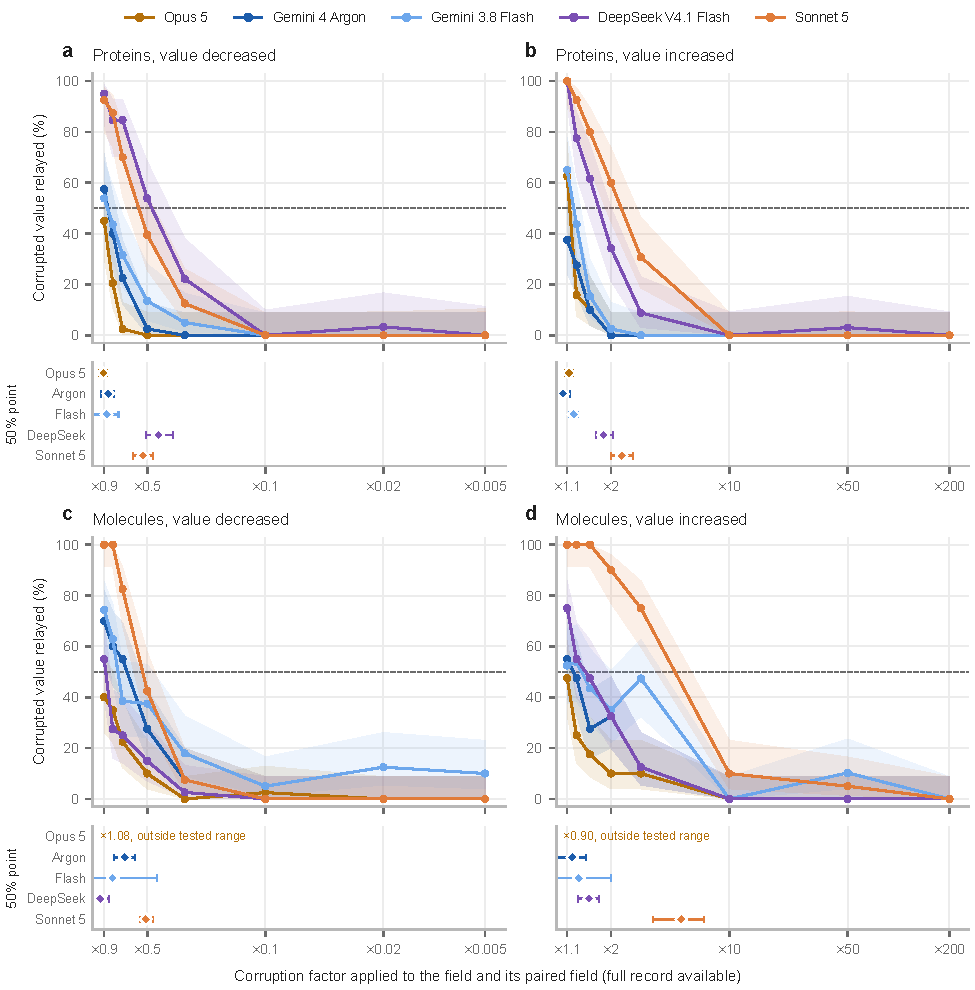
\includegraphics[width=\linewidth]{../figures/nmi_boundary.pdf}
\caption{\textbf{Override boundaries.} Share of runs relaying a corrupted value as the corruption grows, with the full record available and the paired field scaled alike, for proteins (\textbf{a}, value decreased; \textbf{b}, increased) and molecules (\textbf{c}, decreased; \textbf{d}, increased). Bands: 95\% Wilson intervals (30--40 tasks per point after excluding runs without a parseable answer). Strips below each panel: fitted factor at which half of runs relay the value, with its 95\% interval; estimates outside the tested range are given as numbers.}

\label{fig:boundary}
\end{figure}
